
\documentclass[12pt]{article} 

\usepackage{geometry}
\geometry{a4paper} 

\usepackage{graphicx} 
\usepackage{enumitem}
\usepackage{booktabs}

\usepackage{float} 
\usepackage{wrapfig} 

\usepackage{amsmath}
\usepackage{amsfonts}
\usepackage{amssymb}
\usepackage{dsfont}

\usepackage{color}
\usepackage{framed}
\definecolor{shadecolor}{RGB}{248,248,248}
\newenvironment{Shaded}{\begin{snugshade}}{\end{snugshade}}

\usepackage{xcolor}
\usepackage{listings}
\usepackage{caption}
\DeclareCaptionFont{white}{\color{white}}
\DeclareCaptionFormat{listing}{%
  \parbox{\textwidth}{\colorbox{gray}{\parbox{\textwidth}{#1#2#3}}\vskip-2pt}}
\captionsetup[lstlisting]{format=listing,labelfont=white,textfont=white}
\lstset{frame=lrb,xleftmargin=\fboxsep,xrightmargin=-\fboxsep}


\linespread{1.2} 

\setlength\parindent{0pt} % Uncomment to remove all indentation from paragraphs




\begin{document}

\title{\textbf{Multiple Linear Regression II}}
\author{Hyunwoo Gu}
\date{}

\maketitle


\section*{Review \& Corrections}

\begin{itemize}
	\item Increasing Dimensions in Linear Regression
	\item Sum of Squares Principle
	\item Orthogonal Regression
\end{itemize}

\subsection*{Increasing Dimensions in Linear Regression}

\subsection*{Sum of Squares Principle}

\subsection*{Support Vector Regression}

\begin{figure}[h!]
	\centering
	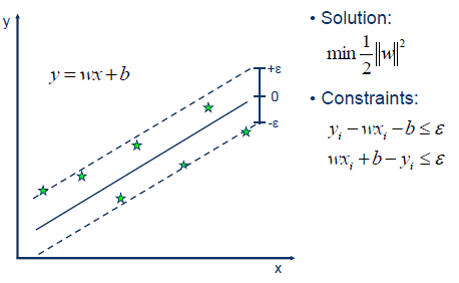
\includegraphics[scale=0.5]{SVR.png}
\end{figure}

\subsection*{Orthogonal Regression}


\pagebreak
\setcounter{section}{3}
%----------------------------------------------------------------------------------------
%	Section 4
%----------------------------------------------------------------------------------------
\section{Confidence Intervals in Multiple Regression}

\subsection{Confidence Intervals on the Regression Coefficients}

Assuming $\epsilon_i \overset{iid}{\sim} N(0, \sigma^2)$,

$$
\begin{aligned}
\hat{\beta} &\sim N\left( \beta, \sigma^2 (X'X)^{-1} \right) \\[8pt]
\hat{\beta_j} &\sim N\left( \beta_j, \sigma^2 C_{jj} \right)
\end{aligned}
$$

thus we have

$$
\frac{ \hat{\beta_j} - \beta_j }  { \sqrt{ \hat{\sigma^2} C_{jj} } } \sim t(n-p)
$$

Based on the above formula, we may define a \textbf{$100(1-\alpha)$ percent confidence interval for the regression coefficient $\beta_j$} as 

$$
\hat{\beta_j} - t_{\alpha/2}(n-p) \mathrm{se}(\hat{\beta_j}) \le \beta_j \le \hat{\beta_j} + t_{\alpha/2}(n-p) \mathrm{se}(\hat{\beta_j})
$$

where $ \mathrm{se}(\hat{\beta_j}) := \sqrt{\hat{\sigma^2} C_{jj}}$, the standard error of the regression coefficient $\hat{\beta_j}$. 



\subsection{CI Estimation of the Mean Response}


By defining $x_0 := [1, x_{01}, \cdots, x_{0k}]'$, the fitted value at the point is $\hat{y_0} = x_0' \hat{\beta}$, an unbiased estimator of $\mathbb{E} (y | x_0)$. 

Note that $\mathrm{Var} (\hat{y_0}) = \sigma^2 x_0' (X'X)^{-1} x_0$. Therefore, a \textbf{$100(1-\alpha)$ percent confidence interval on the mean response} at the point $x_{01}, \cdots, x_{0k}$ is as follows.

$$
\hat{y}_0 - t_{\alpha/2}(n-p) \sqrt{\hat{\sigma^2} x_0' (X'X)^{-1} x_0 } \le \mathbb{E} (y | x_0) \le \hat{y}_0 + t_{\alpha/2}(n-p) \sqrt{\hat{\sigma^2} x_0' (X'X)^{-1} x_0 }
$$




\subsection{Simultaneous Confidence Intervals on Regression Coefficients}

Note that the \textbf{one-at-a-time intervals}, where the confidence coefficient $1 - \alpha$ indicates the proportion of correct statements, result when repeated random samples are selected and the appropriate interval estimate is constructed for each sample. Some problems require that \textbf{several confidence/prediction intervals be contructed using the same sample data}. A set of confidence or prediction intervals that are \textbf{all true simultaneously with probability $1 - \alpha$} are called \textbf{simultaneous/joint confidence/prediction intervals}.

A \textbf{joint confidence region} for the multiple regerssion model parameters $\beta$ is 

$$
\begin{aligned}
\frac{ \left( \hat{\beta} - \beta \right)' X' X (\hat{\beta} - \beta)   }{p MS_{Res}} &\sim F(p, n-p) \\[12pt]
p \left\{   \frac{ \left( \hat{\beta} - \beta \right)' X' X (\hat{\beta} - \beta)   }{p MS_{Res}} \le F_\alpha(p, n-p) \right\} &= 1 - \alpha
\end{aligned}
$$

thus we could say a \textbf{$100 (1 - \alpha) $ percent joint confidence region} for all the parameters in $\beta$ is

$$
\frac{ \left( \hat{\beta} - \beta \right)' X' X (\hat{\beta} - \beta)   }{p MS_{Res}}  \le F_\alpha(p, n-p)
$$

which describes an elliptically shaped region. 


\bigskip
There is another general approach for obtaining simultaneous interval estimates of the parameters in a linear regression model. These CIs may be constructed by using

$$
\hat{\beta_j} \pm \Delta \mathrm{se} (\hat{\beta_j})
$$

where the constant $\Delta$ is chosen so that a specified probability that all intervals are correct is obtained. 


\bigskip
In the \textbf{Bonferroni method}, we set $\Delta := t_{\alpha/2} (n-p) $. The probability that all intervals are correct is at least $1 - \alpha$. Notice that the \textbf{Bonferroni confidence intervals} look somewhat like the ordinary one-at-a-time CIs based on the $t$ distribution, except that each Bonferroni interval has a confidence coefficient $1 - \alpha/p$ instead of $1 - \alpha$. 

The confidence ellipse is always a more efficient procedure that the Bonferroni method because the volume of the ellipse is always less than the volume of the space covered by the Bonferroni intervals. 

\bigskip
In the \textbf{Scheffé's S-method}, we set $\Delta := (2F_\alpha (p, np-1))^{1/2}$. 


\bigskip
In the \textbf{maximum modulus $t$ procedure}, we set $\Delta := u_\alpha (p, n-p)$. 

\bigskip
Generally the intervals are \textbf{maximum modulus} $<$ \textbf{Bonferroni} $<$  \textbf{Scheffé's}. 


%----------------------------------------------------------------------------------------
%	Section 5
%----------------------------------------------------------------------------------------
\section{Prediction of New Observations}

A \textbf{point estimate of the future observation} $y_0$ at the point $x_{01}, \cdots, x_{0k}$ is 

$$
\hat{y_0} = x_0' \hat{\beta}
$$


A \textbf{$100(1 - \alpha)$ percent prediction interval} for this future observation is 

$$
\hat{y_0} - t_{\alpha/2}(n-p) \sqrt{ \hat{\sigma^2} (1 + x_0' (X'X)^{1} x_0) } \le y_0 \le \hat{y_0} + t_{\alpha/2}(n-p) \sqrt{ \hat{\sigma^2}}
$$



In multiple linear regression we notice that the plot of actual versus predicted response is much improved when compared to the plot for the simple linear regression model. 




Finally, the response is predicted with better precision in the multiple linear model. 


\setcounter{section}{7}
%----------------------------------------------------------------------------------------
%	Section 8 
%----------------------------------------------------------------------------------------
\section{Hidden Extrapolation in Multiple Regression}

\begin{figure}[h!]
	\centering
	\includegraphics[scale=0.8]{HiddenExtrapolate.png}
\end{figure}

One must be careful abour \textbf{extrapolating} beyond the region containing the original observations, since it is very possible that a model that fits well in the region of the original data will perform poorly outside that region. In multiple regression, it is easy to inadvertently extrapolate, since the \textbf{levels of the regressors jointly define the region containing the data}. 

Define the \textbf{smallest convex set} containing all of the original $n$ data points $(x_{i1}, x_{i2}, \cdots, x_{ik})$ as the \textbf{regressor variable hull(RVH)}. 

The diagonal elements of $h_{ii}$ of the hat matrix $X(X'X)^{-1}X'$ are useful in detecting \textbf{hidden extrapolation}. The values of $h_{ii}$ depend both on the Euclidean distance of the point $x_i$ from the centroid and on the density of the points in the RVH. 

In general, $h_{max}$ will lie on the boundary of the RVH in a region of the $x$ space where the density of the observations is relatively low. The set of $x$ such that 

$$x' (X'X)^{-1} x \le h_{max}$$

is an \textbf{ellipsoid} enclosing all points inside the RVH. Thus, if we are interested in prediction or estimation at the point $x_0 = [1, x_{01}, x_{02}, \cdots, x_{0k}]$, the location of that point relative to the RVH is reflected by

$$h_{00}= x_0' (X'X)^{-1} x_0 $$.

Note that 

\begin{itemize}
	\item \textbf{Extrapolation} : points with $h_{00} > h_{max}$ are outside the ellipsoid
	\item \textbf{Intrapolation} : points with $h_{00} < h_{max}$ are inside the ellipsoid
\end{itemize}

\pagebreak
%----------------------------------------------------------------------------------------
%	Section 9 
%----------------------------------------------------------------------------------------
\section{Standardized Regression Coefficients}

Usually, it is difficult to directly compare regression coefficients because the magnitude of $\hat{\beta}_j$ reflects the units of measurement of the regressor $x_j$. Generally, \textbf{the units of $\beta_j$} are \textbf{units of $y$}/\textbf{units of $x_j$}. For this reason, it is sometimes helpful to work with scaled regressor and response variables that produce \textbf{dimensionless regression coefficients}, i.e. \textbf{standardized regression coefficients}.


\bigskip
% Unit Normal Scaling
In \textbf{Unit Normal Scaling}, we use

$$
\begin{aligned}
z_{ij} &:= \frac{x_{ij} - \bar{x}_j }{s_j} \\
y_i^\ast &:= \frac{y_i - \bar{y} }{s_y} \\[10pt]
s_j^2 &:= \frac{ \sum_i (x_{ij} - \bar{x}_j)^2 }{ n-1 } \\
s_y^2 &:= \frac{ \sum_i (y_i - \bar{y})^2 }{ n-1 }
\end{aligned}
$$

thus all of the scaled regressors and reponses have sample mean zero and variance $1$. Using the new variables, the regression model becomes

$$
\begin{aligned}
y_i^\ast &= b_1 z_{i1} + \cdots + b_k z_{ik} + \epsilon_i \\[8pt]
\hat{b} &= (Z'Z)^{-1}Z' y^{\ast}
\end{aligned}
$$

where $\hat{b}$ is the least-squares estimator of $b$, and note that $\hat{b}_0 = \bar{y}^\ast = 0$. 



\pagebreak
% Unit Normal Scaling
In \textbf{Unit Length Scaling}, we use

$$
\begin{aligned}
w_{ij} &= \frac{ x_{ij} - \bar{x}_j }{ s_{jj}^{1/2} } \\[8pt]
y_i^0 &= \frac{y_i - \bar{y} }{SS_T^{1/2}} \\[10pt]
S_{jj} &:= \sum_i (x_{ij} - \bar{x}_j)^2
\end{aligned}
$$

In this scaling, each new regressor $w_j$ has mean $\bar{w}_j = 0$ and length $\sqrt{ \sum_i ( w_{ij} - \bar{w}_j)^2 } = 1 $. Thus, the vector of LS regression coefficients is

$$
\hat{b} = (W'W)^{-1}W' y^0
$$

In the unit length scaling, the $W'W$ is in the form of a \textbf{correlation matrix},

$$
\begin{aligned}
W'W &=  \begin{bmatrix}  1      & r_{12} & r_{13} & \cdots & r_{1k} \\
						 r_{12} & 1      & r_{23} & \cdots & r_{2k} \\
						 r_{13} & r_{23} & 1      & \cdots & r_{3k} \\
						 \vdots & \vdots & \vdots &        & \vdots \\
						 r_{1k} & r_{2k} & r_{3k} & \cdots & 1      \\\end{bmatrix}\\[12pt]
r_{ij} &= \frac{S_{ij}}{(S_{ii} S_{jj} )^{1/2}}
\end{aligned}
$$

where $r_{ij}$ is the simple correlation between regressors $x_i$ and $x_j$. Similarly, 

$$
W'
$$

The \textbf{standardized regression coefficients} $\hat{b}$ have relationship 

$$
\begin{aligned}
\hat{\beta}_j &= \hat{b}_j \left( \frac{SS_T}{S_{jj}} \right)^{1/2} \\[8pt]
\hat{\beta}_0 &= \bar{y} - \sum_j^k \hat{\beta}_j \bar{x}_j
\end{aligned}
$$

Many multiple regression algorithms use the \textbf{unit length scaling} in order to reduce problems arising from round-off errors in $(X'X)^{-1}$. These round-off errors may be very serious if the original variables differ considerably in magnitude. 

Note that the standardized regression coefficients are still \textbf{partial regression coefficients}, and $b_j$ are affected by the range of values for the regressor variables. Consequently, it may be dangerous to use the magnitude of $\hat{b}_j$ as a measure of the relative importance of regressor $x_j$. 



%----------------------------------------------------------------------------------------
%	Section 10
%----------------------------------------------------------------------------------------
\section{Multicollinearity}

Multicollineary implies near-linear dependence among the regressors. The regressors are the columns of the $X$ matrix, so an \textbf{exact linear dependence} would result in a \textbf{singular $X'X$}.

\textbf{$X'X$ is invertible $\Leftrightarrow$ $\mathrm{rank}(X) = p$}. 

\bigskip

\begin{Shaded}
\textbf{Proof}

\bigskip
Note that the condition $\mathrm{rank}(X) = p$ forces $p \le n$. $\forall v \in \mathbb{R}^p$, $Xv = 0 \Leftrightarrow X'Xv = 0$, since if $X'Xv = 0$ then $v' X' Xv=0$ then $Xv=0$. 

\smallskip
If $\mathrm{rank} (X) < p$, there exists $v \neq 0 \in \mathbb{R}^p$ such that $X v = 0$. Since this implies $X'Xv=0$, $X'X$ cannot be invertible.

\smallskip
On the other hand, if $\mathrm{rank}(X) = p$, then null space of $X'X$ is trivial, since null space of $X$ is trivial and generally $\mathrm{null}(X) = \mathrm{null}(X'X)$. Since it is square, $X'X$ is invertible
\end{Shaded}

Note that $X'X$ : invertible $\Leftrightarrow$ $X$ has a left inverse, which is $(X'X)^{-1}X'$ and is called \textbf{Moore-Penrose pseudoinverse} of $X$.  


Suppose we use the \textbf{unit length} scaling so that $X'X$ matrix will be in the form of a correlation matrix.






\subsection*{More on Variance Inflation Factors}

If $x_j$ is nearly orthogonal to the remaining regressors, $R_j^2$ is small and $C_{jj}$ is close to unity, while if $x_j$ is nearly linearly dependent on some subset of the remaining regressors, $R_j^2$ is near unity and $C_jj$ is large.  Note that $VIF_j = C_{jj} = (1 -R_j^2)^{-1}$, where $C_{jj}$ can be viewed as the factor by which the variance $\hat{\beta}_j$ is increased due to near-linear dependences among the regressors. 

BTW, the length of the normal theory confidence interval on the $j$th regression coefficient may be written as 

$$
L_j = 2 (C_{jj} \sigma^2)^{1/2} t_{\alpha/2} (n-p-1)
$$

and the length of the corresponding interval based on an \textbf{orthogonal reference design} with the same sample size and RMS values as the original design is 

$$
L^\ast = 2 \sigma t_{\alpha/2} (n-p-1)
$$

so note that $L_j / L^\ast = C_{jj}^{1/2}$. Thus the square root of the $j$th VIF indicates \textbf{how much longer the confidence interval for the $j$th regression coefficient is because of multicollinearity.} 


\subsection{Eigensystem Analysis of $X'X$}

The \textbf{eigenvalues} of $X'X$, say $\lambda_1, \cdots, \lambda_p$ can be used to measure the extent of multicollinearity in the data. If there are one or more near-linear dependences in the data, then one or more of the characteristic roots will be small, and vice versa. Define the \textbf{condition number} and \textbf{condition indices} of $X'X$, 


$$
\begin{aligned}
\kappa &= \frac{\lambda_{max}}{\lambda_{min}} \\[8pt]
\kappa_j &= \frac{\lambda_{max}}{\lambda_j}
\end{aligned}
$$

If $\kappa$ exceeds $1000$, severe multicollinearity is indicated. 

\textbf{Eigensystem analysis} can also be used to identify the nature of the near-linear dependences in data. $X'X$ matrix may be decomposed as 

$$
X'X = T \Lambda T'
$$

where $\Lambda$ is $p \times p$ diagonal matrix whose main diagonals are the \textbf{eigenvalues} $\lambda_j$ of $X'X$ and $T$ is $p \times t$ orthogonal matrix whose columns are \textbf{eigenvectors} of $X'X$. 


$$
X = UDT'
$$

where $U$ is $n \times p$, $T$ is $p \times p$, $U'U = I_p$, $T'T=I_p$, and $D$ : $p \times p$ diagonal matrix with nonnegative diagonal elements $\mu$. The $\mu_j$ are called the \textbf{singular values} of $X$ and $X = UDT'$ is called the \textbf{singular-value decomposition} of $X$. 

Note that $X'X = (UDT')'(UDT') = TD^2T' = T\Lambda T' $, so that the squares of the singular values of $X$ are the eigenvalues of $X'X$. 

Also, Ill-conditioning in $X$ is reflected in the size of the singular values. The covariance of $\hat{\beta}$ is

$$
\begin{aligned}
\mathrm{Var} (\hat{\beta}) &= \sigma^2 (X'X)^{-1} = \sigma^2 T \Lambda^{-1}T' \\[8pt]
\mathrm{Var} (\hat{\beta}_j) &= \sigma^2 \sum_i^p \frac{t_{ji}^2 }{\mu_i^2} = \sigma^2 \sum_i^p \frac{t_{ji}^2 }{\lambda_i}  \\[10pt]
VIF_j &= \sum_i^p \frac{t_{ji}^2 }{\mu_i^2} = \sum_i^p \frac{t_{ji}^2 }{\lambda_i}  \\[10pt]
\end{aligned}
$$

Clearly, one or more small singular values can dramatically inflate the variance of $\hat{\beta}_j$. 



\pagebreak
%----------------------------------------------------------------------------------------
%	Section 11
%----------------------------------------------------------------------------------------
\section{Why Do Regression Coefficients Have the Wrong Sign?}

Occasionally we find an apparent contradiction of intuition or theory when one or more of the regression coefficients seem to have the \textbf{wrong sign}. 

\bigskip
\textbf{1. The range of some of the regressors is too small.}

Note that $\mathrm{Var} (\hat{\beta_1}) = \sigma^2/S_{xx} = \sigma^2/\sum(x_i - \bar{x})^2$, which is inversely proportional to the \textbf{spread} of the regressor. 

Therefore, if the levels of $x$ are all close together, the variance of $\hat{\beta}_1$ will be relatively large, thus raising the possibility of the sign being wrong. 

\bigskip
\textbf{2. Important regressors have not been included in the model.}

In these cases, the sign is not really wrong. The partial nature of the regression coefficients cause the sign reversal. A partial regression coefficient measures the effect of $x_i$ \textbf{given} that $x_j (i \neq j)$ is also in the model. 


\bigskip
\textbf{3. Multicollinearity is present.}

In effect, severe \textbf{multicollinearity} inflates the variances of the regression coefficients, and this increases the probability that one or more regression coefficients will have the wrong sign. 


\bigskip
\textbf{4. Computational errors have been made.}

Different computer programs handle round-off or truncation problems in different ways. Aside from this, severe multicollinearity causes $X'X$ to be \textbf{ill-conditioned}, which is a source of computational error. 



\pagebreak
%----------------------------------------------------------------------------------------
%	Relative Importance among the features 
%----------------------------------------------------------------------------------------




\pagebreak
%----------------------------------------------------------------------------------------
%	Problems
%----------------------------------------------------------------------------------------

\section*{Problems}
\subsubsection*{Problem 3.33.} Prove that $R^2$ is the square of the correlation between $y$ and $\hat{y}$.
\bigskip


\subsubsection*{Problem 3.35.} Let $x_j$ be the $j$th row of $X$, $X_{-j}$ be the $X$ matrix with $j$th row removed. Show that 

$$
\mathrm{Var}[\hat{\beta}_j] = \sigma^2 [x_j' x_j - x_j' X_{-j} (X_{-j}' X_{-j} )^{-1} X_{-j}' x_j  ]^{-1}
$$

\bigskip

\subsubsection*{Problem 3.37.} Suppose we fit the model $y = X_1 \beta_2 + \epsilon$ when the true model is actually given by $y = X_1 \beta_2 + X_2 \beta_2 + \epsilon$, where $\mathbb{E}(\epsilon) = 0, \mathrm{Var}(\epsilon) = \sigma^2 I $. Find the expected value and variance of the OLS estimate, $\hat{\beta}_1$. Under what conditions is this estimate unbiased?

\bigskip

\subsubsection*{Problem 3.39.} Let $R_j^2$ be the coefficient of determination when we regress the $j$th regressor on the other $k-1$ regressors. Show that the $j$th variance inflation factor may be expressed as 

$$
\frac{1}{1-R_j^2}
$$

\bigskip

We have

$$
\begin{aligned}
\mathrm{Var}(e_i) &= \mathrm{Var}(y_i) + \mathrm{Var}(\hat{y}_i) - 2 \mathrm{Cov}(y_i, \hat{y}_i) \\[8pt]
&= \sigma^2 (1 - 1/n - (x_i - \bar{x})^2/S_{xx})
\end{aligned}
$$




\pagebreak
%----------------------------------------------------------------------------------------
%	Kaggle
%----------------------------------------------------------------------------------------
\section*{Kaggle: On Random Forests}

A \textbf{Random Forest} is an ensemble of Decision Trees, generally trained via the baggin method.

\setcounter{section}{1}
\setcounter{subsection}{0}

\subsection{Decision Trees}

Decision trees are versatile Machine Learning algorithms that can perform both classification and regression tasks. They provide less need to preprocess, are interpretable, and stable.

In CART algorithms, \textbf{Gini impurity} is used, defined as follows.

$$
G_i := 1 - \sum_{k=1}^n p_{i, k}^2
$$

which means the probability of being false in random sampling from a set. 


\subsection{Random Forest}

A group of predictors is called an \textbf{ensemble}. So you could train a group of decision trees, each on a different random subset of the training set. To make predictions, you just obtain the predictions of all individual trees, then predict the class that gets the most votes.

When \textbf{bagging}, some instances may be sampled several times for any given predictor, while others not be sampled at all. The training instances that are not sampled are called \textbf{out-of-bag} instances, which eliminate the need for a separate validation set or cross-validation. 


\subsection{Relative Importance Metrics}

\end{document}